\section{事件与可测结构}
\label{sec:pspace-events}

在有限的古典模型里，样本空间的每个子集都是事件，都可以问概率。木棍上的随机点也能这样处理吗？回答这个问题之前，先看三种情形，它们分别从不同方向说明：事件族需要单独指定，不能默认是样本空间的全部子集。

\paragraph{连续位置}
木棍上的随机点取值于$\Omega=[0,1)$，我们要求区间的概率等于它的长度。由此出发，区间的有限并、补集都有自然的概率；有理数集$\mathbb{Q}\cap[0,1)$是可数个单点之并，也应当有概率。可是能不能给$[0,1)$的\emph{每个}子集都指定一个“长度”，同时保持区间长度不变、平移不变和可数可加？卷四给出了否定的回答：用选择公理构造的Vitali集在这些要求下无法赋值，可参考\BookChapterRef{chap:measure}{卷四第5章“测度”}。所以对连续位置，我们只能对一部分子集谈概率。

\paragraph{混合的取值}
等待时间$W$以概率$0.3$恰好取$0$，其余$0.7$的质量按密度$0.7\,\mathrm{e}^{-t}$铺在$(0,\infty)$上。要描述它，单点$\{0\}$必须是事件，各种区间也必须是事件，而且两种事件要能一起运算，例如“$W$等于$0$或大于$2$”。概率表只处理可数个点，密度只处理区间上的积分，事件族必须同时容纳两者。

\paragraph{不同的记录方式}
掷两枚骰子，样本空间是$36$个有序对$(i,j)$。如果观察者只被告知点数和$S=i+j$，他能判断哪些事件是否发生？“$S=7$”可以，“$S$是偶数”也可以，但“第一枚是$1$”不行：$S=7$时第一枚可能是$1$，也可能是$6$。图~\ref{fig:pspace-dice-partitions}(a)中红框是事件“第一枚是$1$”，它横跨了点数和不同的六个格子，只取其中各一个格子。在同一个样本空间上，可以判断的事件族取决于观察到了什么。

\begin{BookInlineFigure}
  \centering
  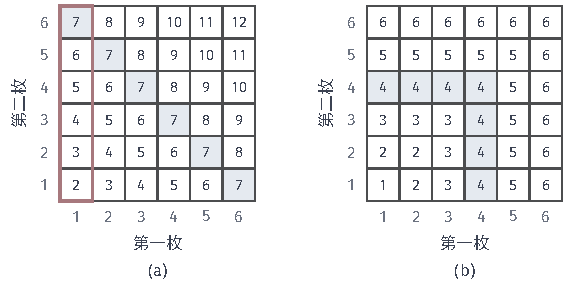
\includegraphics[width=96mm]{figures/07-probability/02-measure-theoretic-probability/tikz/pspace-dice-partitions/figure.pdf}
  \caption{同一个样本空间上的两种记录。每个格子是一个有序结果$(i,j)$。(a)格内是点数和$S$，浅蓝格子组成$\{S=7\}$；红框是事件“第一枚是$1$”，它把$S$取值相同的格子拆开了，只知道$S$无法判断它是否发生。(b)格内是较大点数$M$，浅蓝的L形区域是$\{M=4\}$。}
  \label{fig:pspace-dice-partitions}
\end{BookInlineFigure}

三种情形的共同点是：样本空间$\Omega$回答“可能出现哪些结果”，另需一个子集族回答“可以对哪些结果集合问概率”。前者是试验的描述，后者是我们愿意且能够提问的范围。

\paragraph{事件族应满足的运算}
什么样的子集族适合做事件族？从提问的角度看，至少有三条要求。整个$\Omega$应当是事件，“某个结果出现了”总能回答。若能判断$A$是否发生，也就能判断$A$不发生，所以事件族对补集封闭。若能逐一判断$A_1,A_2,\dots$是否发生，就应当能判断“其中至少一个发生”，所以事件族对可数并封闭。

为什么要求可数并而不只是有限并？第~\ref{chap:classical-probability}章抛硬币直到出现正面，事件“迟早出现正面”是“第$k$次首次出现正面”对$k=1,2,\dots$之并；有理数集是可数个单点之并。概率论中的极限陈述，例如“平均值收敛”，也都要用可数次并与交写出来。只要求有限并的事件族装不下这些事件。

这三条恰好是卷四$\sigma$代数的定义。设$\mathcal{F}$是$\Omega$的子集族，满足：
\begin{enumerate}
  \item $\Omega\in\mathcal{F}$；
  \item 若$A\in\mathcal{F}$，则$A^{\mathrm{c}}\in\mathcal{F}$；
  \item 若$A_1,A_2,\dots\in\mathcal{F}$，则$\bigcup_{k}A_k\in\mathcal{F}$。
\end{enumerate}
称$\mathcal{F}$为$\Omega$上的$\sigma$代数，$(\Omega,\mathcal{F})$为可测空间。由补集和可数并还能得到可数交：
\[
  \bigcap_{k}A_k=\Bigl(\bigcup_{k}A_k^{\mathrm{c}}\Bigr)^{\mathrm{c}}\in\mathcal{F},
\]
以及$\varnothing=\Omega^{\mathrm{c}}\in\mathcal{F}$、差集$A\setminus B=A\cap B^{\mathrm{c}}\in\mathcal{F}$。

\begin{definition}[事件]
\label{def:pspace-event}
设$(\Omega,\mathcal{F})$是可测空间。$\mathcal{F}$中的集合称为事件，$\mathcal{F}$称为\term{事件族}（family of events）。
\end{definition}

从此“事件”是一个相对于$\mathcal{F}$的概念。$\Omega$的子集未必是事件；同一个$\Omega$配上不同的$\mathcal{F}$，描述的是同一组结果上不同的提问范围。第一部分在有限或可数的$\Omega$上取全部子集，在实轴上只对区间及其有限并谈概率，都是这里的特例或其中的一部分。

\paragraph{有限样本空间上的事件族}
$\Omega$有限时，$\sigma$代数有一个具体的样子：它把$\Omega$分成若干块，事件恰好是若干块的并。块的构造是取包含某个点的所有事件之交。对$\omega\in\Omega$，令
\begin{equation}
  A(\omega)=\bigcap\{A\in\mathcal{F}:\omega\in A\},
  \label{eq:pspace-atom}
\end{equation}
称为$\omega$所在的\term{原子}（atom）。$\mathcal{F}$是有限族，所以这是有限交，$A(\omega)\in\mathcal{F}$。它是包含$\omega$的最小事件。

\begin{lemma}[有限样本空间上的$\sigma$代数]
\label{lem:pspace-finite-atoms}
设$\Omega$有限，$\mathcal{F}$是$\Omega$上的$\sigma$代数。则不同的原子两两不交，它们构成$\Omega$的一个划分；$\mathcal{F}$中每个事件都是若干个原子之并。若原子共有$k$个，则$\mathcal{F}$恰有$2^{k}$个事件。
\end{lemma}

\begin{proof}
先证两个原子要么相同、要么不交。设$A(\omega)\cap A(\omega')\neq\varnothing$。若$\omega\notin A(\omega')$，则$A(\omega)\setminus A(\omega')$是包含$\omega$的事件，且比$A(\omega)$小，与$A(\omega)$的最小性矛盾。所以$\omega\in A(\omega')$，于是$A(\omega)\subseteq A(\omega')$。对称地$A(\omega')\subseteq A(\omega)$，两者相同。

再证每个事件是原子之并。设$A\in\mathcal{F}$。对每个$\omega\in A$，$A$是包含$\omega$的事件，所以$A(\omega)\subseteq A$。于是
\[
  A=\bigcup_{\omega\in A}A(\omega),
\]
右边是若干个原子之并。反过来，原子都是事件，有限个事件之并仍是事件。所以$\mathcal{F}$恰由原子的各种并组成。$k$个两两不交的原子，每个选或不选，给出$2^{k}$个不同的并。
\end{proof}

在骰子的例子里，只知道$S$的观察者能判断的事件族，以$S$的$11$个取值对应的格子组为原子，即图~\ref{fig:pspace-dice-partitions}(a)中的各条反对角线。由引理~\ref{lem:pspace-finite-atoms}，这个事件族有$2^{11}=2048$个事件，而$36$个结果的全部子集有$2^{36}$个。“第一枚是$1$”不是原子之并，所以不在其中。只知道较大点数$M$的观察者，原子是图~\ref{fig:pspace-dice-partitions}(b)中的$6$个L形区域，事件族有$2^{6}=64$个事件。

\paragraph{生成的事件族}
实际建模时，我们通常只知道几个“想问的事件”，并不想逐一列出整个$\sigma$代数。卷四给出了办法：对$\Omega$的任意子集族$\mathcal{C}$，包含$\mathcal{C}$的所有$\sigma$代数之交仍是$\sigma$代数，它是包含$\mathcal{C}$的最小$\sigma$代数，记作$\sigma(\mathcal{C})$。它就是从$\mathcal{C}$出发、反复做补集与可数并所能得到的全部事件。

最简单的情形是一个事件$A$。包含$A$的$\sigma$代数必须含有$\Omega$、$A$和$A^{\mathrm{c}}$，因而含有$\varnothing$，而这四个集合已经对补集和并封闭，所以
\[
  \sigma(\{A\})=\{\varnothing,A,A^{\mathrm{c}},\Omega\}.
\]
两个相交的事件$A,B$把$\Omega$切成四块（图~\ref{fig:pspace-generated-events}）。四块都要在$\sigma(\{A,B\})$中，而它们的各种并已经构成$\sigma$代数，所以$\sigma(\{A,B\})$恰有$2^{4}=16$个事件。

\begin{BookInlineFigure}
  \centering
  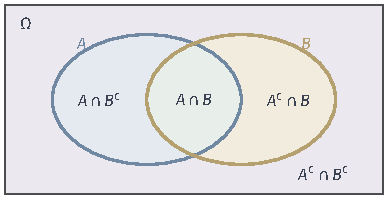
\includegraphics[width=66mm]{figures/07-probability/02-measure-theoretic-probability/tikz/pspace-generated-events/figure.pdf}
  \caption{两个事件$A$（蓝框）与$B$（黄框）把$\Omega$切成四个原子：$A\cap B^{\mathrm{c}}$（浅蓝）、$A\cap B$（浅绿）、$A^{\mathrm{c}}\cap B$（浅黄）和$A^{\mathrm{c}}\cap B^{\mathrm{c}}$（浅紫）。$\sigma(\{A,B\})$由这四块的全部$16$种并组成。}
  \label{fig:pspace-generated-events}
\end{BookInlineFigure}

对木棍上的随机点，想问的事件是区间。由区间生成的$\sigma$代数就是卷四的Borel $\sigma$代数，记作$\mathcal{B}([0,1))$。它不仅含有区间，还含有单点$\{x\}=\bigcap_n[x,x+1/n)$、有理数集、无理数集以及Cantor集等用可数次运算得到的集合。我们无法把它的成员一一列出，但对每个具体的集合，只要说出它怎样由区间经可数次运算得到，就知道它是事件。实轴上的$\mathcal{B}(\mathbb{R})$、$d$维空间上的$\mathcal{B}(\mathbb{R}^{d})$同理，它们也可以分别由半直线$(-\infty,x]$、左下象限$(-\infty,x_1]\times\cdots\times(-\infty,x_d]$生成。

表~\ref{tab:pspace-event-families}汇总了本章常用模型的样本空间与事件族。

\begin{BookInlineTable}
  \centering
  \caption{常用模型的样本空间与事件族}
  \label{tab:pspace-event-families}
  \begin{tabular}{lll}
    \toprule
    模型 & 样本空间$\Omega$ & 事件族$\mathcal{F}$ \\
    \midrule
    两枚骰子 & $36$个有序对 & 全部子集 \\
    只知道点数和 & $36$个有序对 & $\sigma(S)$，$2^{11}$个事件 \\
    木棍上的点 & $[0,1)$ & $\mathcal{B}([0,1))$ \\
    等待时间$W$ & $\mathbb{R}$ & $\mathcal{B}(\mathbb{R})$ \\
    \bottomrule
  \end{tabular}
\end{BookInlineTable}

表中的$\sigma(S)$是由点数和生成的事件族，第~\ref{sec:pspace-random-objects}节对一般的观测给出它的定义。
